\documentclass[12pt]{article}
\renewcommand{\thesubsubsection}{\alph{subsubsection}}
% Fonts and Encoding
\usepackage[utf8]{inputenc}
\usepackage[T1]{fontenc}
\usepackage{ebgaramond} % Beautiful serif font
\usepackage{microtype}
\usepackage{float}
\usepackage{graphicx}
\usepackage{hyperref}
\usepackage{xcolor}
\usepackage[
    colorlinks=true,
    linkcolor=black,
    urlcolor=blue,       % default URL color
    citecolor=black
]{hyperref}

% Page Setup (A4 format)
\usepackage[a4paper,top=2.5cm,bottom=2.5cm,left=3cm,right=3cm]{geometry}
\usepackage{setspace}
\setstretch{1.3}

% Colors and Graphics
\usepackage{xcolor}
\definecolor{myblue}{HTML}{2C3E50}
\definecolor{mygray}{HTML}{F8F9FA}
\definecolor{darkgray}{gray}{0.2}

% Section Styling
\usepackage{titlesec}
\titleformat{\section}
  {\normalfont\Large\bfseries\color{myblue}}
  {\thesection}{1em}{}
\titleformat{\subsection}
  {\normalfont\large\bfseries\color{darkgray}}
  {\thesubsection}{1em}{}

% Code block style
\usepackage{listings}
\lstset{
  backgroundcolor=\color{mygray},
  basicstyle=\ttfamily\small,
  frame=single,
  framerule=0pt,
  rulecolor=\color{gray},
  xleftmargin=1em,
  xrightmargin=1em,
  breaklines=true,
  tabsize=2,
  showstringspaces=false
}

% Header/Footer
\usepackage{fancyhdr}
\pagestyle{fancy}
\fancyhf{}
\lhead{\textit{Large Language Model}}
\rhead{\thepage}
\renewcommand{\headrulewidth}{0pt}

% Graphics
\usepackage{graphicx}

% Document info
\title{The Speaking Machine}
\author{Idrissi Kandri Badreddine}
\date{\today}

\begin{document}

\begin{titlepage}
  \centering
  \vspace*{1.5cm}
  
  {\Huge \bfseries The Speaking Machine \par}
  \vspace{1.5em}
  
  {\Large \textit{Understanding Large Language Models} \par}
  \vspace{3em}
  
  {\large \textbf{Author:} Idrissi Kandri Badreddine \par}
  \vspace{1em}
  
  {\large \today \par}
  \vspace{1em}
  
  
\includegraphics[width=0.8\textwidth]{images/llm0.jpg}
  
  \vfill
\end{titlepage}


\newpage
\thispagestyle{empty}

\vspace*{4cm}

\begin{center}
    \Huge\textbf{Author's Note}
\end{center}

\vspace{1cm}

\noindent
This Technical Booklet was written and realized by \textbf{Idrissi Kandri Badreddine} during my first year of engineering studies in \textit{Information Systems and Big Data}.

\vspace{0.5cm}

\noindent
It represents my very first research project, focused on providing a clear and structured understanding of \textbf{Large Language Models (LLMs)}. Through this work, I aim to break down the complexity behind these models and make them accessible, especially to students and newcomers in the world of artificial intelligence.

\vspace{0.5cm}

\noindent
What makes this Booklet special is the passion and dedication I put into every page. I truly hope you find it insightful, useful, and inspiring particularly if you're taking your first steps into the fascinating world of AI.

\vspace{1cm}

\noindent
\textbf{Redaction:} \LaTeX \\
\textbf{Visuals and Schemas:} Designed using \texttt{app.diagrams.net}

\vfill

\begin{flushright}
    \textit{Idrissi Kandri Badreddine} \\
    \textit{Student Engineer in Big Data and Information Systems}
\end{flushright}

\newpage
\vspace*{3cm}
\hypersetup{hidelinks}
\tableofcontents
\newpage
\vspace*{4cm}
\section{Introduction}

In recent years, Large Language Models (LLMs) have revolutionized the way humans interact with machines. From answering questions and writing essays to generating code and engaging in natural conversations, these models are increasingly becoming essential tools in our daily lives. But behind the simplicity of typing a question and getting an instant response lies a complex and carefully engineered process one that blends mathematics, linguistics, data, and deep learning.

This Booklet aims to demystify that process.

Rather than treating LLMs as black boxes, we will open them up and explore what truly happens inside. We'll walk step-by-step through the life of an LLM from how it is trained on massive text corpora to how it generates fluent, context-aware responses at inference time. Along the way, we’ll break down core concepts such as tokenization, embeddings, attention mechanisms, loss functions, and gradient-based optimization, using clear explanations and intuitive examples.

Whether you are a curious learner, a student of AI, or an aspiring developer, this book is designed to give you both the theoretical understanding and the practical insight needed to appreciate the inner workings of modern language models. 

Let us begin our journey into the fascinating world of LLMs where language meets intelligence, and where machines learn to speak.
\newpage

\section{Definition}
A Large Language Model (LLM) is a type of AI model trained on vast amounts of data using deep learning techniques, particularly Transformer architectures, with the goal of producing logical output from a given input

\vspace{1em}
\hspace{-0.8cm}
\begin{center}
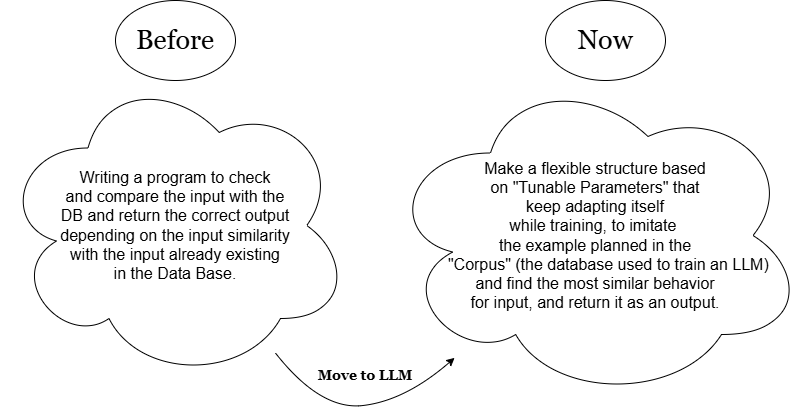
\includegraphics[width=1\textwidth]{images/llm1.png}
\end{center}


In Deep Learning: Tunable Parameters = \textbf{Weights}

=>Model Brain - Learn during training - Defines the model behaviors.
\section{Process}
To fully understand all aspects of LLMs, we need to learn about its two main phases: training and inference.

\vspace{3em}
\hspace{-1.4cm}
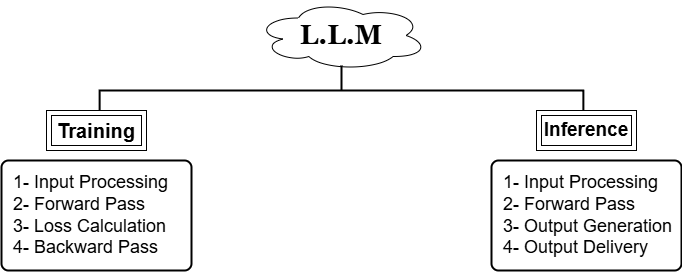
\includegraphics[width=1.1\textwidth]{images/llm2.png}

\newpage
\section{Inside the LLM}
\subsection{Input Processing}
In the input processing phase, there are two steps. The first one is \textbf{Tokenization}, in this step, the model converts every slice of the input into tokens. These slices can be words, punctuation marks, or letters, it all depends on how the model was trained.\\Then comes the \textbf{Embedding} step when the model converts each token into a vector with random numerical values, called an embedding. This vector contains two types of information: the slice’s meaning (without considering the sentence context) and its position in the sentence.

\vspace*{1.5cm}
\hspace{-1.5cm}
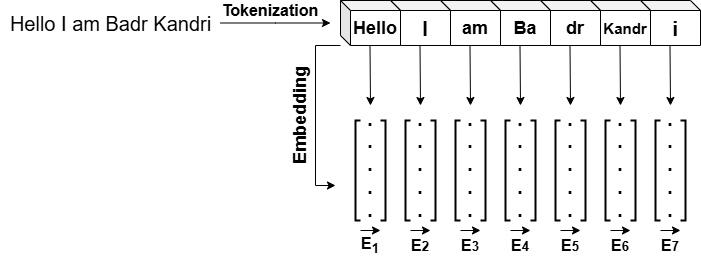
\includegraphics[width=1.1\textwidth]{images/llm3.png}
\vspace*{1.5cm}
\textbf{OBJECTIF:} Adjusting weights by updating the vectors to organize them based on their meaning.


\begin{center}
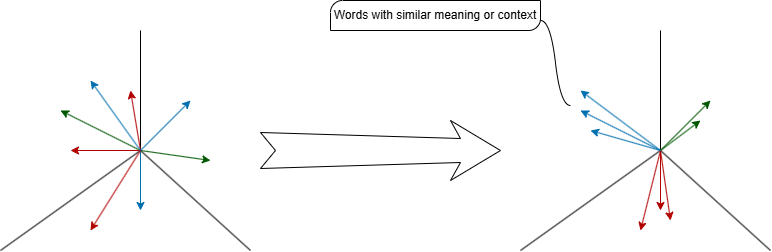
\includegraphics[width=\textwidth]{images/llm4.png}
\end{center}

\newpage

\subsection{Forward Pass}
Forward Pass in an LLM (like ChatGPT) Is the phase where input tokens are passed through the Transformer architecture. After each token is converted into an embedding vector, through multiple layers of self-attention and MLP , the model captures the meaning and context of each token relative to others. The final output is a prediction (next word or full response), generated using the learned relationships all without changing the model’s weights.
\textcolor{blue}{\subsubsection{Self-Attention}}
Self-attention is the step where each word looks at every other word in the sentence to understand their relationships and identify which ones influence its meaning.\\This was a friendly definition of what really happens in this phase. Now, let's dive deeper into what actually happens mathematically and geometrically. And to do that, we’re going to divide it into 8 steps.\\
\textcolor{brown}{\textbf{Step 1:}} Each embedding generates a \textbf{Query vector \overrightarrow{Q}}, which allows it to interact with other embeddings in order to identify those that are most related to it.\\
\begin{center}
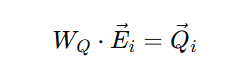
\includegraphics[width=0.4\textwidth]{images/formula1.png}
\end{center}
\textcolor{brown}{\textbf{\\Step 2:}} Each embedding generates a \textbf{Key vector \overrightarrow{k}} which contains the information needed to respond to queries from other embeddings.\\
\begin{center}
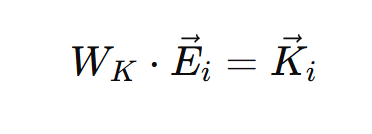
\includegraphics[width=0.4\textwidth]{images/formula2.png}
\end{center}
\textcolor{brown}{\textbf{\\Step 3:}} Each \textbf{\(\overrightarrow{k_i}\)} is multiplied by every \textbf{\(\overrightarrow{Q_i}\)}, producing dot product values. Large values imply a strong correlation between the embeddings.\\so we say that \textbf{the key \(\overrightarrow{k_i}\) attends to the query \(\overrightarrow{Q_i}\)}.\\Geometrically, this corresponds to the two vectors being nearly aligned.\\
\newpage

\textcolor{brown}{\textbf{\\Step 4: (Masking)}} The dot product values are then multiplied by a masking matrix that sets certain values to zero. This prevents a token from attending to future positions and forces it to predict the next token based only on past tokens. This mechanism helps the model better understand the context of the input, leading to more accurate predictions.\\

\textcolor{brown}{\textbf{\\Step 5: }} Each embedding generates a \textbf{Value vector \overrightarrow{V}}, which defines the information to be added to the original embedding \( \vec{E_i} \) in order to obtain the updated embedding \( \vec{E_i'} \).\\
\begin{center}
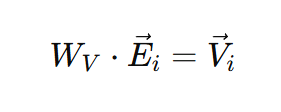
\includegraphics[width=0.3\textwidth]{images/formula3.png}
\end{center}
The \( W_V \) is the \textbf{Value Matrix}, and it is composed of an augmentation matrix and a reduction matrix, and the \( V_i \) is called the \textbf{Weight}.

\textcolor{brown}{\textbf{\\Step 6: }} The result from Step 4 (Masking) is then normalized into probabilities using the \textbf{Softmax} function, and subsequently multiplied by the value vectors.\\
\begin{center}
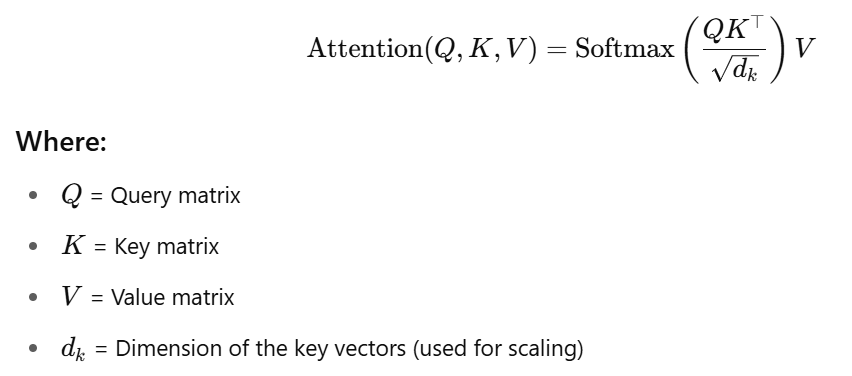
\includegraphics[width=\textwidth]{images/formula4.png}
\end{center}
This produce an \textbf{Attention Pattern:\\}
\begin{center}
    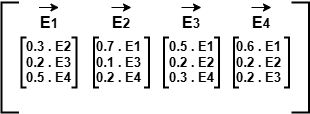
\includegraphics[width=0.5\textwidth]{images/llm5.png}
\end{center}

\textcolor{brown}{\textbf{\\Step 7: }} Generate the contextualized embeddings.\\
\begin{center}
    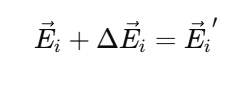
\includegraphics[width=0.3\textwidth]{images/formula5.png}
\end{center}
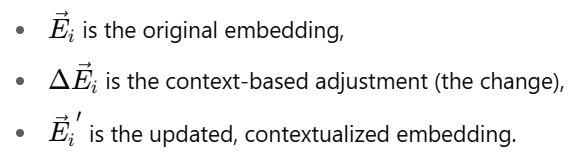
\includegraphics[width=0.7\textwidth]{images/formula6.png}

\textcolor{brown}{\textbf{\\Step 8: }} Generate the Matrix of contextualized embeddings (one row for each token).

\begin{center}
    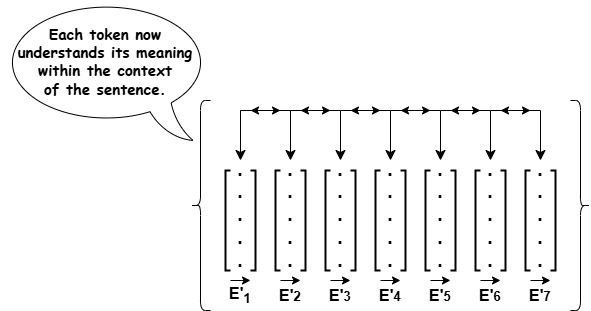
\includegraphics[width=0.8\textwidth]{images/llm6.png}
\end{center}



\textcolor{red}{\textbf{\\=> RECAP:}} Steps 1 to 8 describe the single-head attention process.
However, in practice, this process happens multiple times in parallel and that’s what we call multi-head attention.\\


\begin{center}
    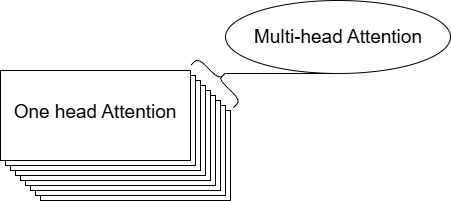
\includegraphics[width=0.8\textwidth]{images/llm7.png}
\end{center}

\textcolor{red}{\textbf{\\Attention output :}} a Matrix

\newpage

\textcolor{blue}{\subsubsection{Multi-Layer Perceptron (MLP)}}
After linking the embeddings with one another through the attention mechanism, the next step is to connect each embedding with the factual knowledge encoded in the LLM’s corpus. This is precisely the role of the Multi-Layer Perceptron (MLP) component.\\
We will now explain how the LLM proceeds to enrich each embedding with external knowledge by following a series of well-defined steps. To make this process more intuitive, we summarize it in the following explanatory diagram:\\
\vspace*{0.4cm}
\begin{center}
    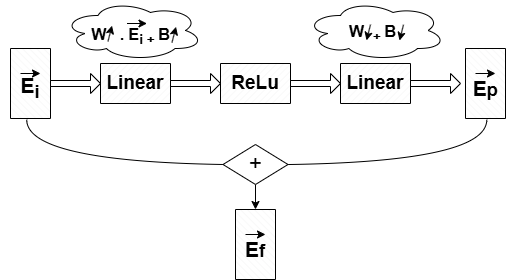
\includegraphics[width=0.8\textwidth]{images/llm8.png}
\end{center}

\textcolor{teal}{Linear (1st):} Define the direction of the embedding vector in the embedding space.

\textcolor{teal}{ReLU (Rectified Linear Unit):} Reduce all the negative values to 0.

\textcolor{teal}{Linear (2nd):} Define the vector that will be added to the input vector.

\textcolor{blue}{\subsubsection{Layer Normalization}}
This step is crucial to stabilize the tokens’ embedding vectors and ensure consistent scale and better training or inference performance.\\And we will do this by normalizing the MLP output:\textbf{\(\overrightarrow{E_f}\)}\\
\begin{center}
    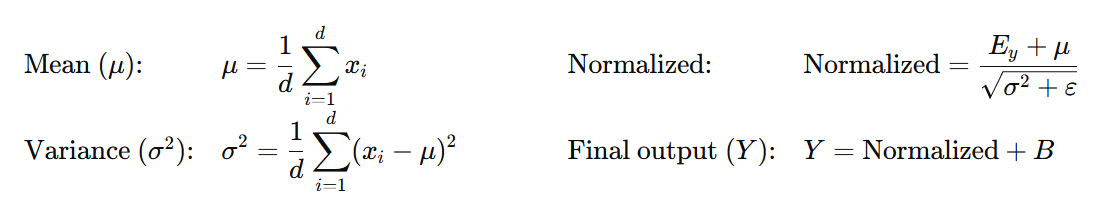
\includegraphics[width=\textwidth]{images/formula7.png}
\end{center}

\textcolor{red}{\\Important:} This step is also between the self-attention and MLP.

\begin{center}
    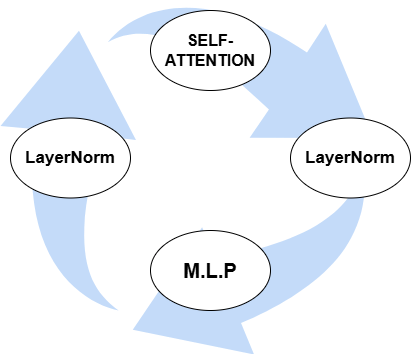
\includegraphics[width=0.5\textwidth]{images/llm9.png}
\end{center}

This cycle repeats n times based on the model, and in the final iteration, the last layer-norm produces a final matrix. The desired output is the last vector of this matrix, referred to as the final hidden state.\\
\begin{center}
    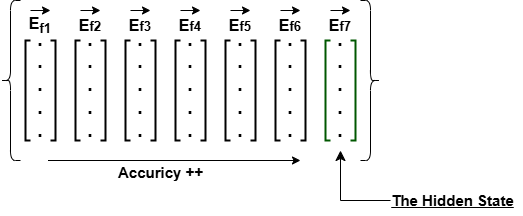
\includegraphics[width=0.9\textwidth]{images/llm10.png}
\end{center}
The model uses an unembedding matrix to transform the hidden state into a probability distribution over the vocabulary:
\begin{center}
    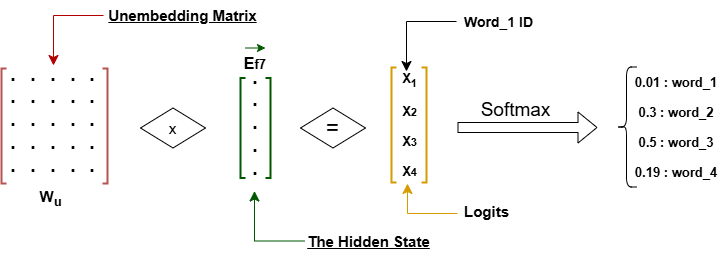
\includegraphics[width=1.1\textwidth]{images/llm13.png}
\end{center}

\newpage
\vspace*{0.2cm}
\subsection{The Softmax Function}

Following the forward pass, the hidden state becomes a vector of numbers within the interval $ ]-\infty, +\infty[ $. Since predictions should represent probabilities, how can we transform this vector into a list of probabilities for the next token corresponding to each element?\\ This is where softmax is utilized in large language models (LLMs) to normalize the vector into a list of probabilities between [0 , 1].\\so how does this function operate?
\begin{center}
    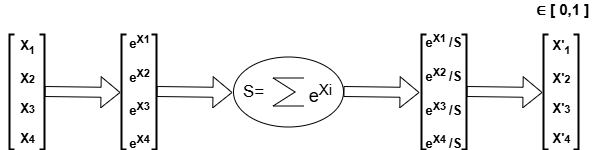
\includegraphics[width=\textwidth]{images/llm11.png}
\end{center}

After applying the softmax function, all values in the vector now range between 0 and 1, allowing us to interpret them as probabilities that the large language model (LLM) uses to predict the next token. However, this approach has a limitation: the softmax function often produces values that are significantly different from one another. This makes it easy for the LLM to consistently select the token with the highest probability, which can reduce creativity to zero, as the model tends to predict the same word repeatedly.

To address this issue, researchers introduced a new parameter called "temperature" to the formula. Temperature is a small value that helps minimize the differences between the vector's values, resulting in more uniform probabilities. This encourages the LLM to select different tokens each time, rather than always choosing the highest one, thereby enhancing the model's creativity. To implement this temperature adjustment, each value in the vector is divided by the temperature parameter. Typically, a temperature value less than 1 increases focus on the most likely tokens, while a value greater than 1 promotes more diverse and creative outputs.\\

\begin{center}
    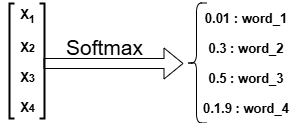
\includegraphics[width=0.7\textwidth]{images/llm12.png}
\end{center}

\newpage
\vspace*{1cm}
The first three steps are crucial in every process involving an LLM: tokenization, embedding, and attention-based processing. However, the rest of the process differs depending on whether the model is in \textbf{training} or \textbf{inference} (usage) mode.\\
In this section, we will tackle each process separately, starting first with the training phase.
\subsection{LLM Training}
To train an LLM, the next step is to take the list of predicted probabilities and compute the loss, which measures how "surprised" the model is when its predictions differ from the correct tokens. This loss quantifies the error between the predicted and actual tokens.\\Then, the model performs backpropagation, which calculates the gradients (the direction and magnitude) of change needed, and uses these gradients to update the model's weights.\\This process helps the model improve its predictions over time.
\textcolor{blue}{\subsubsection{Loss Calculation}}
To measure how "surprised" the model is when its predictions differ from the correct tokens, we compute the \textbf{Cross-Entropy Loss}, which quantifies the difference between the predicted probability distribution and the actual (true) distribution.\\The cross-entropy loss is defined by the following formula:
\begin{center}
    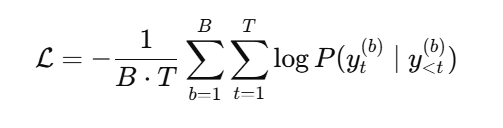
\includegraphics[width=0.7\textwidth]{images/formula8.png}
\end{center}

\begin{center}
    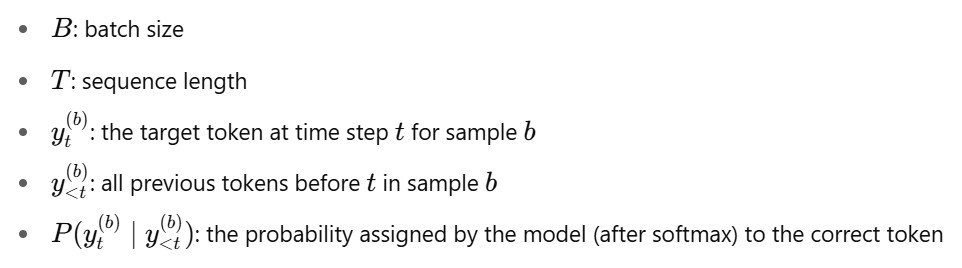
\includegraphics[width=\textwidth]{images/formula9.png}
\end{center}
\newpage

\textcolor{blue}{\subsubsection{Backpropagation}}
Now that the model knows how far off its predictions are compared to the correct tokens in the corpus ''thanks to the loss value'' it needs to adjust itself accordingly. If the prediction was wrong, the model should change its internal parameters(weights) if it was right, it should reinforce that behavior. This process is known as optimization.

There are many optimization algorithms used in deep learning, such as \textbf{SGD}, \textbf{Adam}, and others. However, to keep things simple, we can summarize the core idea through the concept of \textbf{gradient} calculation.

By computing the gradient (the derivative of the loss with respect to each weight), the model determines how much each weight contributed to the error. The gradient acts like a guide, telling the model how to update its weights in order to reduce future errors and make better predictions over time.

\begin{center}
    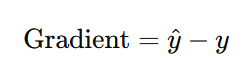
\includegraphics[width=0.5\textwidth]{images/formula10.png}
\end{center}
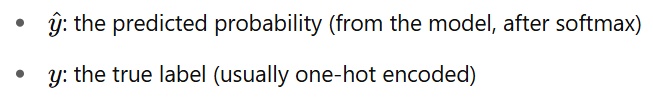
\includegraphics[width=0.8\textwidth]{images/formula11.png}

\vspace*{1cm}

That’s it, you now have a solid understanding of what happens behind the scenes during the training of a large language model. From tokenization and embedding to attention mechanisms, loss calculation, gradient computation, and weight updates, we’ve explored how the model gradually learns to predict language accurately. But training is only half the story.\\To complete our journey through the architecture and functioning of LLMs, we now shift our focus to the \textbf{inference phase}, the stage where the model is actually used in real-world applications. This is the typical scenario where a user types a prompt and instantly receives a coherent, often intelligent, response.\\But what really happens under the hood when you interact with an LLM?
How does the model interpret your input, generate meaningful text, and appear to communicate like a human?
What mechanisms guide its generation of sentences, word by word, from learned patterns?

These are the questions we’ll dive into next to uncover how inference works, how the model produces text in real-time, and how it becomes a powerful tool for human-AI interaction.


\subsection{LLM Inference}
The inference step is the phase where the LLM is already trained and begins using what it has learned to assist humans with various tasks such as answering questions, generating content, or solving problems. Since the model has completed its training, we no longer evaluate or adjust its predictions, we assume it has been sufficiently trained to produce accurate and meaningful responses. Technically, the inference process involves two main stages: output generation and output delivery. In the output generation stage, the model receives the probabilities list from the \textbf{forward pass} step, processes it, and generates a response internally in the form of numerical vectors. Then, in the output delivery stage, these numerical outputs are decoded and converted into natural human language that the user can understand. In the following section, we will explore the first stage of inference: output generation.

\textcolor{blue}{\subsubsection{Output Generation}}
At this stage, each number in the probability distribution returned by the softmax function corresponds to a specific token (word or symbol) from the model's vocabulary(Corpus). The model selects one of these tokens based on a \textbf{decoding strategy} that reflects how it was trained, such as \textbf{Greedy search}, \textbf{Sampling}, or \textbf{Beam search}. Once a token is chosen, the model identifies its corresponding \textbf{ID} in the vocabulary. This token ID becomes the \textbf{final output} for that time step and is appended to the sequence of previously generated tokens.\\This updated sequence, now including the newly generated token, becomes the input for the next generation step. Through this iterative process, the model generates text \textbf{token by token} until it reaches a \textbf{stopping condition}, such as a maximum length or an end-of-sequence token.

\textbf{====> Exemple of Output: \textcolor{teal}{\large ID=325("and")}}

\textcolor{blue}{\subsubsection{Output Delivery}}

Now, let's tackle the final step of inference: \textbf{output delivery}. In the previous step, the model repeatedly generated tokens one by one, appending each new token ID to the input sequence until a complete sequence was formed. This process continues based on a stopping condition defined during training. As a result, the model produces a sequence of token IDs:
\textcolor{teal}{\large\[
[\textbf{325},\ \textbf{2023},\ \textbf{2003},\ \textbf{1037},\ \textbf{2742},\ \textbf{102}]
\]}
Each of these IDs corresponds to a word or symbol in the model's vocabulary.\\
\newpage
Okay, so now the model has completed the generation process and knows exactly which tokens it will add to the user's input. However, these tokens are still in the form of numerical IDs, which are not understandable to humans. To transform this sequence into natural language, the model must go through a final stage called \textbf{detokenization}. This process involves four key steps:
\begin{enumerate}
  \item \textbf{ID to Token Mapping:} Each token ID is mapped back to its corresponding token (subword, word, or symbol) using the model’s vocabulary. \textcolor{red}{ID ==> Word}
  \item \textbf{Token Merging:} If the tokenizer used subword units, adjacent tokens are merged to reconstruct the original words. \textcolor{red}{Play + ing ==> Playing}
  \item \textbf{Text Normalization:} Punctuation, spacing, and casing are corrected to ensure the output resembles fluent natural language.
  \item \textbf{Final Output Rendering:} The resulting string is prepared for display or returned to the user as the final response.
\end{enumerate}

\section{Conclusion}

In this Technical Booklet, we have explored in depth the internal functioning of Large Language Models (LLMs), covering both the \textbf{training} and \textbf{inference} phases. During the training phase, we saw how the model learns to understand and generate language through a series of critical steps: tokenization, embedding, attention mechanisms, probability prediction, loss computation, gradient calculation, and weight updates. This process allows the model to gradually improve its ability to predict the next token in a sequence, based on vast amounts of text data.

Once the model is trained, it enters the inference phase the stage where it is actually used by end users. We explained how, during inference, the model receives an input, generates outputs token by token through decoding strategies, and finally converts its internal numerical predictions into human-readable text. This final step involves detokenization, which transforms token IDs into coherent natural language.

Together, these two phases, training and inference represent the complete lifecycle of a large language model, from learning patterns in data to producing intelligent, human-like responses in real time. Understanding this full pipeline is essential not only for building effective language systems, but also for appreciating the remarkable complexity and design behind modern AI communication tools.





\section{Contact}

Connect with me on :\href{https://www.linkedin.com/in/badreddine-idrissi-kandri-365438329/}{\textcolor{blue!80!black}{\textbf{  LinkedIn}}} \\
Check out my projects on :\href{https://github.com/BadrKandri}{\textcolor{gray}{\textbf{  GitHub}}}

\end{document}
